In this section, we describe the N-body simulations used in this study, the process of generating convergence maps, the incorporation of shape and measurement noise, and the techniques employed for patch extraction in covariance analysis.

\section{Initial condition}
\subsection{Primordial Power Spectrum}
Primodial power spectrum is defined as:
\begin{equation}
    P_p(k) = A \left(\frac{k}{k_*}\right)^{n_s - 1}
\end{equation}
where $A$ is the amplitude of the power spectrum, $k$ is the wavenumber, $k_*$ is the pivot scale, and $n_s$ is the spectral index. The power spectrum describes the distribution of matter in the universe and is an essential ingredient in cosmological simulations.
As the universe evolves, various physical processes (like radiation pressure, baryon-photon interactions, and dark matter dynamics) affect the growth of perturbations. These effects are encapsulated in the transfer function $T(k)$, which describes the evolution of the power spectrum from the early universe to the present day. The power spectrum at redshift $z$ is given by
\begin{eqnarray}
    P(k; z) &=& P_p(k) T^2(k, z) D^2(z)  \\
    P(k; z = 0)&=& P_p(k) T^2(k, z=0) 
\end{eqnarray}
where $D(z)$ is the linear growth factor, which describes the growth of perturbations in the linear regime. 
The evolution of cosmological perturbations is governed by the Boltzmann equations for each species. For example, for cold dark matter (CDM), the perturbation equation is given by
\begin{equation}
    \ddot{\delta_m} + 2H\dot{\delta_m} - 4\pi G \rho_m \delta_m = 0
\end{equation}
where $\delta_m$ is the density contrast, $H$ is the Hubble parameter, and $\rho_m$ is the total matter density. 

In a FLRW universe, the linear growth facttor is given by:
\begin{equation}
    D(a) = \frac{5 \Omega_m a}{2} \int_0^1 \frac{da'}{a'^3 H(a')^3}
\end{equation}
The transfer function $T(k)$ is computed using the CAMB code \citep{2000ApJ...538..473L}.

\subsection{Initial Conditions}
\subsubsection{Initial Density Field}
Express the density contrast in terms of its Fourier components:
\begin{equation}
    \delta(\mathbf{x}) = \int \frac{d^3k}{(2\pi)^3} \tilde{\delta}(\mathbf{k}) e^{i\mathbf{k} \cdot \mathbf{x}}
\end{equation}
Assuming the density field is a Gaussian random field, each Fourier mode $\tilde{\delta}(\mathbf{k})$ is a complex Gaussian random variable with zero mean and variance $P(k)$:
\begin{eqnarray}
    \tilde{\delta}(\mathbf{k}) &=& A(\mathbf{k}) + iB(\mathbf{k}) \\
    \langle A(\mathbf{k}) \rangle = \langle B(\mathbf{k}) \rangle &=& 0 \\
    \langle A(\mathbf{k}) A(\mathbf{k'}) \rangle = \langle B(\mathbf{k}) B(\mathbf{k'}) \rangle &=& \frac{P(k)}{2} \delta_D(\mathbf{k} - \mathbf{k'}) \\
    \langle A(\mathbf{k}) B(\mathbf{k'}) \rangle &=& 0
\end{eqnarray}
where $\delta_D$ is the Dirac delta function. The density field is then obtained by taking the inverse Fourier transform of $\delta(\mathbf{k})$.
\subsubsection{Initial Displacement Field}
Under the Zel'dovich approximation, the initial displacement field $\Psi(\mathbf{x})$ is linearly related to the initial density field $\delta(\mathbf{x})$:
\begin{equation}
    \Psi(\mathbf{x}) = - \nabla \Phi(\mathbf{x}) 
\end{equation}
\begin{equation}
    \nabla^2 \Phi = \delta(\mathbf{x})
\end{equation}
In Fourier space, the displacement field is given by:
\begin{eqnarray}
    - k^2 \tilde{\Phi}(\mathbf{k}) &=& \tilde{\delta}(\mathbf{k}) \nonumber \\
    \tilde{\Psi}(\mathbf{k}) &=& -i\mathbf{k} \tilde{\Phi}(\mathbf{k}) = i\mathbf{k} \frac{\tilde{\delta}(\mathbf{k})}{k^2} \nonumber \\
    \Psi(\mathbf{x}) &=& \int \frac{d^3k}{(2\pi)^3} i\mathbf{k} \frac{\tilde{\delta}(\mathbf{k})}{k^2} e^{i\mathbf{k} \cdot \mathbf{x}}
\end{eqnarray}

\subsubsection{Initial Positions and Velocities}
Assuming that particles start in a uniform grid in Lagrangian (initial) coordinates $\mathbf{q}$, the initial positions $\mathbf{x}$ is given by:
\begin{equation}
    \mathbf{x}(\mathbf{q}) = \mathbf{q} + \Psi(\mathbf{q})
\end{equation}
Under the Zel'dovich approximation, the initial velocities $\mathbf{v}$ are proportional to the displacement field:
\begin{eqnarray}
    \mathbf{v}(\mathbf{x}) &=& a H f \Psi(\mathbf{x}) \nonumber \\
    \tilde{\mathbf{v}}(\mathbf{k}) &=& a H f i\mathbf{k} \frac{\tilde{\delta}(\mathbf{k})}{k^2} \nonumber \\
    \mathbf{v}(\mathbf{x}) &=& i a H f\int \frac{d^3k}{(2\pi)^3} \frac{\mathbf{k}}{k^2} \tilde{\delta}(\mathbf{k}) e^{i\mathbf{k} \cdot \mathbf{x}}
\end{eqnarray}
where $f = d\ln D/d\ln a$ is the growth rate of structure formation.

\section{Simulation Basics}
Numerical simulations are indispensable tools in physics and astronomy for investigating complex systems of interacting particles, such as galaxies, star clusters, and the large-scale structure of the Universe. The inherent complexity and nonlinearity of these systems render analytical solutions impractical or intractable, thereby necessitating the application of numerical methods. This section provides a comprehensive overview of $N$-body simulations commonly employed to study the large-scale structure of the cosmos.

To address the computational challenges posed by the long-range nature of gravitational interactions, significant efforts in numerical cosmology since the 1980s have focused on developing algorithms that reduce the need for global communication across the entire computational domain. These algorithms include mesh-based methods, tree codes, and multipole expansions~\citep{1981csup.book.....H}. Figure~\ref{fig:particle-count} illustrates the number of particles utilized in selected $N$-body simulations employing such techniques. The symbols and colors in the figure denote the gravitational solvers used: particle-particle-particle-mesh (P$^3$M) and adaptive P$^3$M (AP$^3$M); parallel or vectorized P$^3$M; Tree codes; TreePM; and particle-mesh methods with adaptive mesh refinement (PM AMR).

Owing to advancements in computational algorithms and software optimization, the number of particles in cosmological simulations has increased at a rate surpassing that achievable with direct summation methods. Notably, since 1990, a super-exponential growth trend has been observed for gravity-only simulations, as indicated by the quadratic regression in Figure~\ref{fig:particle-count}. This acceleration cannot be solely attributed to improvements in computational hardware performance and reflects significant methodological innovations~\citep{leclercq2020}.

\begin{figure}
    \centering
    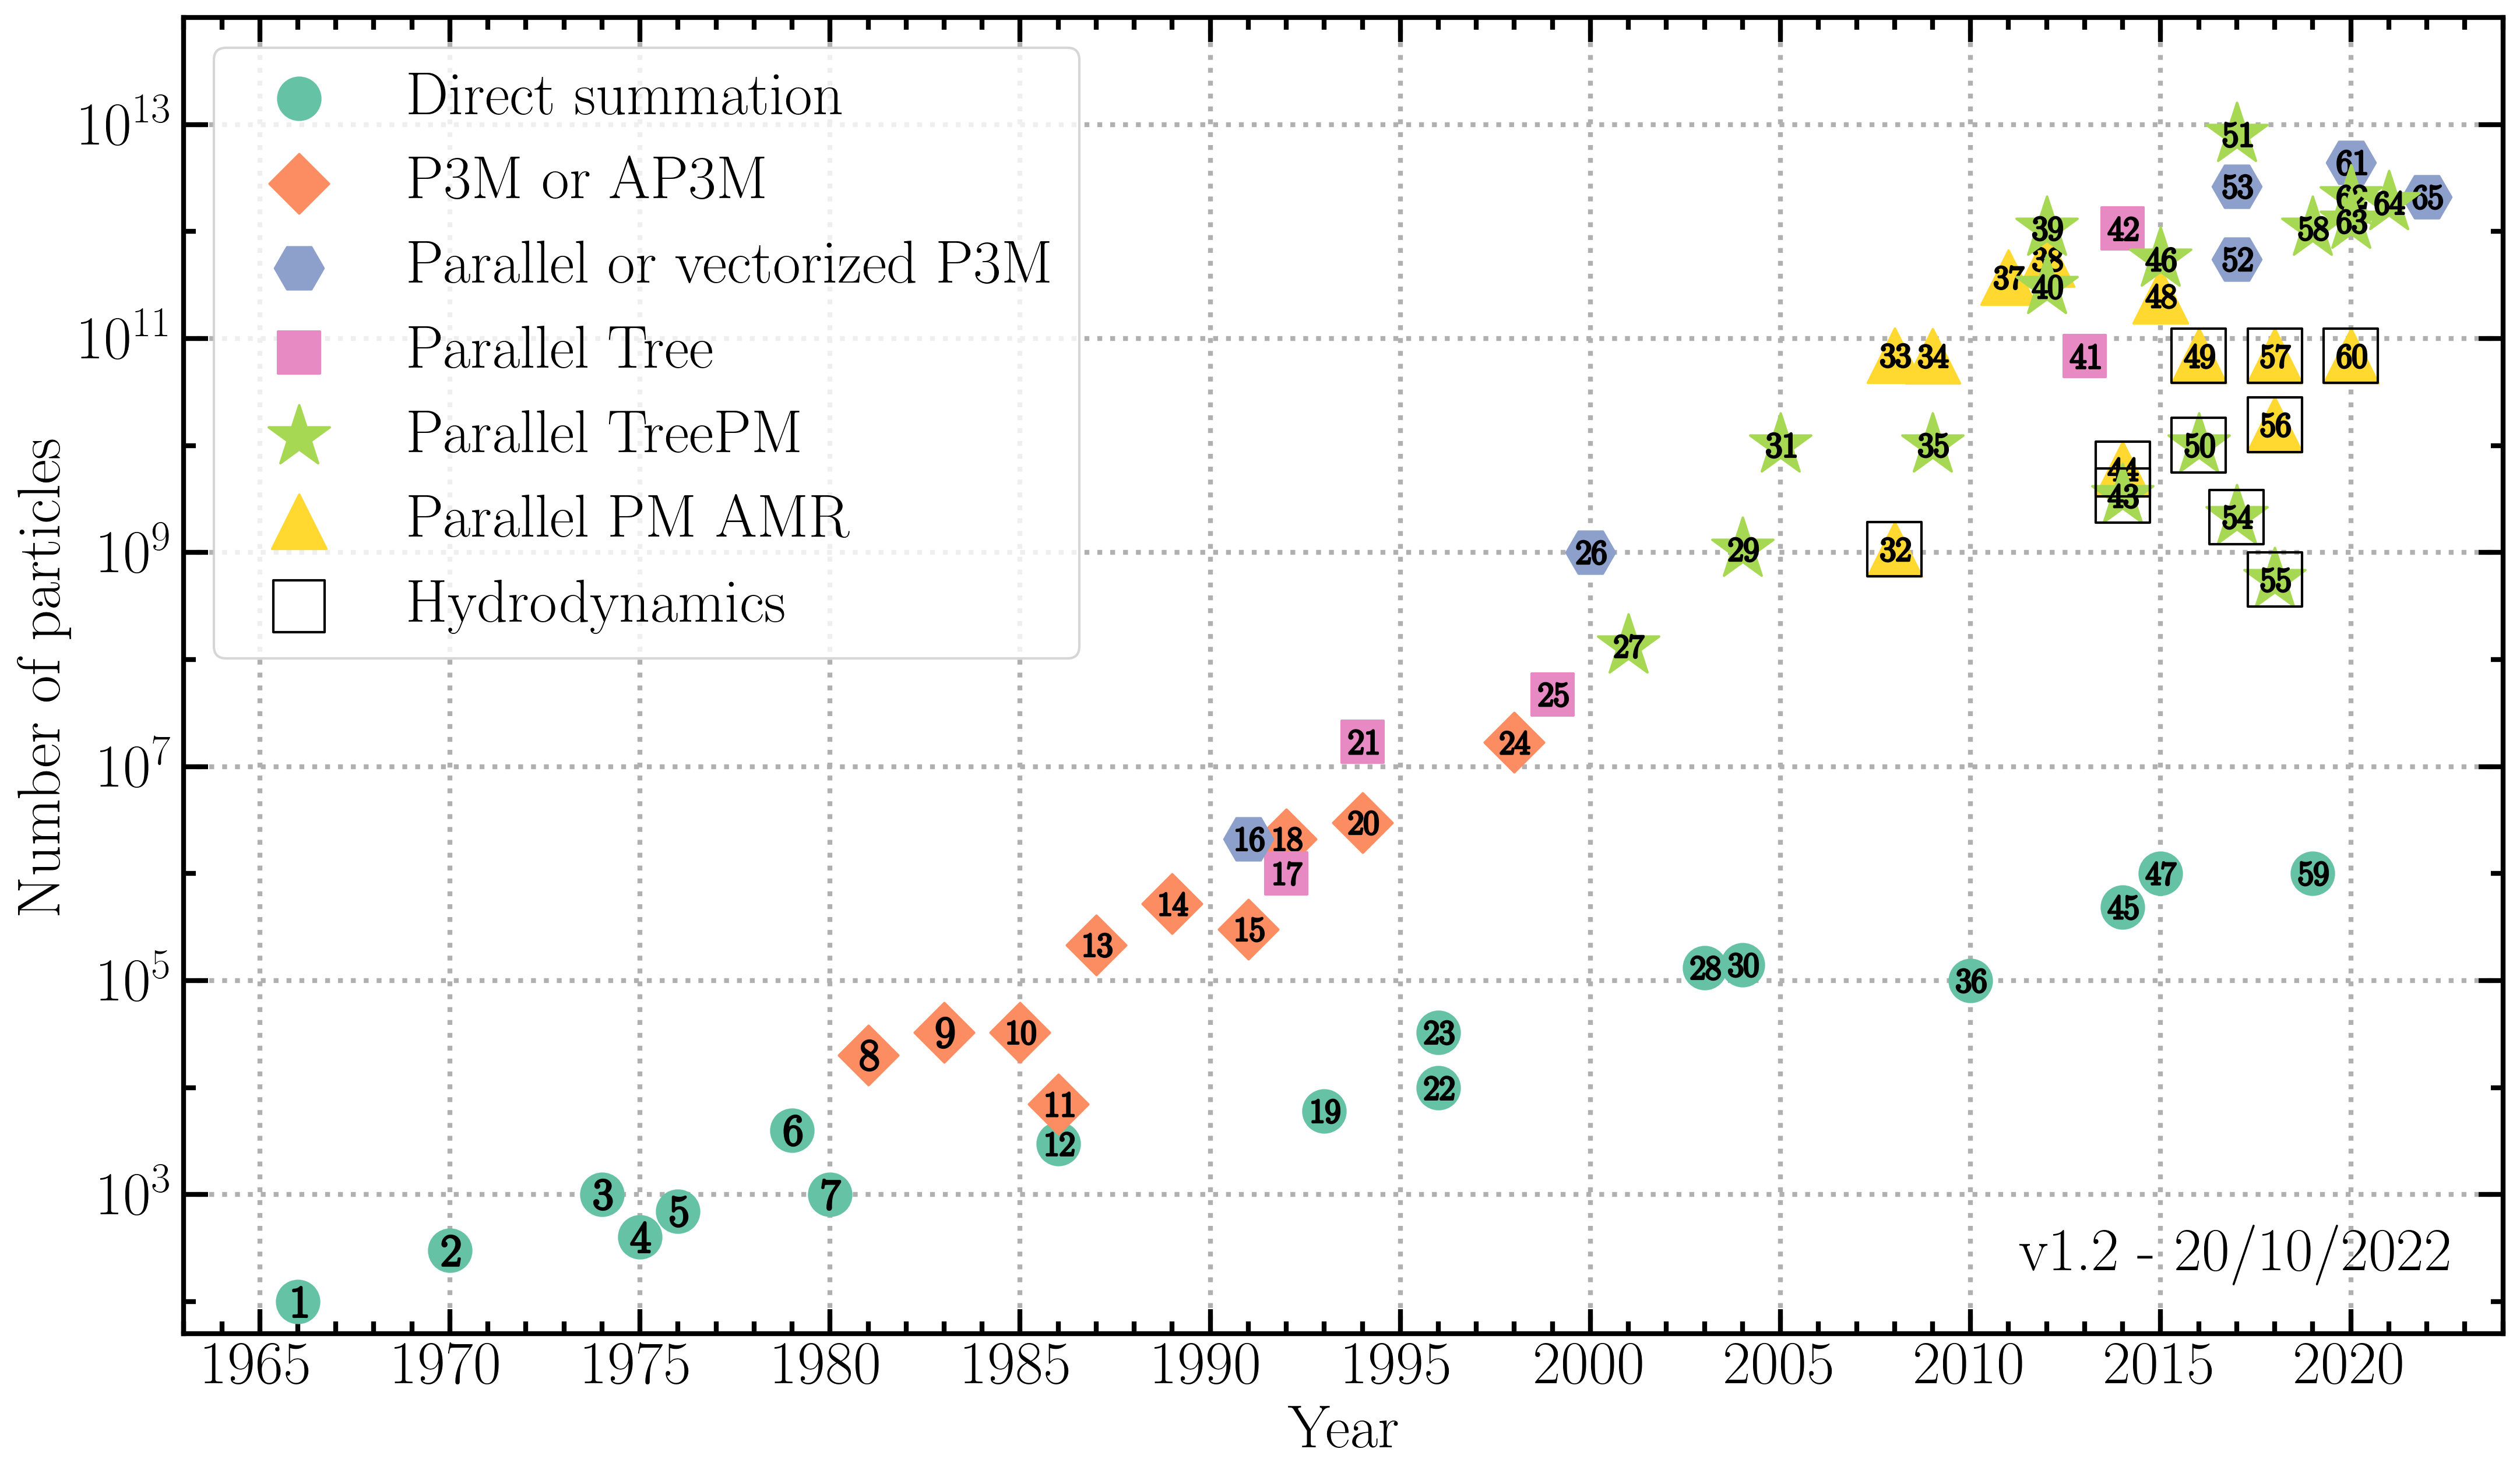
\includegraphics[width=0.6\textwidth]{figures/Moore_law_cosmosims.png}
    \caption{Evolution of the number of particles used in $N$-body simulations as a function of the year of publication~\citep{leclercq2020}. The symbols and colors indicate the gravitational solver employed: P$^3$M and adaptive P$^3$M (AP$^3$M); parallel or vectorized P$^3$M; Tree codes; TreePM; and particle-mesh methods with adaptive mesh refinement (PM AMR). Hydrodynamic simulations are represented by black squares.}
    \label{fig:particle-count}
\end{figure}

\subsection{Direct Summation}
Direct Summation computes gravitational forces between all pairs of particles directly. This method scales with $\mathcal{O}(N^2)$, making it computationally intensive for large $N$. Each particle $i$ is characterized by its position $\mathbf{r}_i$, velocity $\mathbf{v}_i$, and mass $m_i$.

The algorithm proceeds through the following steps at each time step $t$:
\begin{enumerate}
    \item \textbf{Compute Forces:}
    \[
    \mathbf{F}_i = G m_i \sum_{\substack{j=1 \\ j \neq i}}^{N} \frac{m_j (\mathbf{r}_j - \mathbf{r}_i)}{\|\mathbf{r}_j - \mathbf{r}_i\|^3}
    \]
    
    \item \textbf{Update Particle States:}
    \[
    \mathbf{v}_i(t + \Delta t) = \mathbf{v}_i(t) + \frac{\mathbf{F}_i}{m_i} \Delta t, \quad \mathbf{r}_i(t + \Delta t) = \mathbf{r}_i(t) + \mathbf{v}_i(t + \Delta t) \Delta t
    \]
    
    \item \textbf{Advance Time:}
    \[
    t \leftarrow t + \Delta t
    \]
\end{enumerate}

\subsection{Particle-Mesh (PM) Method}
Particle-Mesh (PM) methods approximate gravitational forces by mapping particles onto a grid and solving for the gravitational potential. This approach reduces the computational cost to $\mathcal{O}(N + M \log M)$, where $M$ is the number of grid points. PM methods efficiently handle large-scale simulations but tend to smooth out small-scale forces, potentially sacrificing accuracy at smaller scales.

The algorithm proceeds through the following steps at each time step $t$:
\begin{enumerate}
    \item \textbf{Assign Particles to Grid:} See Section~\ref{sec:mass-assignment}.
    
    \item \textbf{Compute Density Field:}
    \[
    \rho(\mathbf{x}) = \sum_i m_i W(\mathbf{x} - \mathbf{r}_i) \quad \text{(where $W$: Interpolation Kernel)}
    \]
    
    \item \textbf{Solve Poisson's Equation:}
    \[
    \nabla^2 \Phi = 4\pi G \rho
    \]
    
    \item \textbf{Compute Gravitational Field:}
    \[
    \mathbf{E} = -\nabla \Phi
    \]
    
    \item \textbf{Update Particle States:}
    \[
    \mathbf{v}_i(t + \Delta t) = \mathbf{v}_i(t) + \mathbf{E}_i \Delta t, \quad \mathbf{r}_i(t + \Delta t) = \mathbf{r}_i(t) + \mathbf{v}_i(t + \Delta t) \Delta t
    \]
    
    \item \textbf{Advance Time:}
    \[
    t \leftarrow t + \Delta t
    \]
\end{enumerate}

\subsection{Particle-Particle Particle-Mesh (P3M) Method}
The Particle-Particle Particle-Mesh (P3M) method combines direct summation for short-range force calculations with the Particle-Mesh (PM) approach for long-range interactions. This hybrid technique maintains the $\mathcal{O}(N \log N)$ complexity of PM methods while achieving higher accuracy for close particle interactions by explicitly computing particle-particle (PP) forces. Key considerations in the P3M method include the selection of mesh size, the softening parameter $\epsilon$, and the management of force resolution to balance computational efficiency and accuracy.

The algorithm proceeds through the following steps at each time step $t$:

\begin{enumerate}
    \item \textbf{Long-Range Forces (PM):}
    Compute the long-range gravitational forces using the Particle-Mesh approach:
    \[
    \mathbf{F}_{\text{long},i} = m_i \mathbf{E}_{\text{long}}(\mathbf{r}_i)
    \]
    where $\mathbf{E}_{\text{long}}$ is the gravitational field derived from the mesh-based potential.
    
    \item \textbf{Short-Range Forces (Direct Summation):}
    \begin{enumerate}[label={(\alph*)}]
        \item \textbf{Neighbor Search:}
        For each particle $i$, identify neighboring particles $j$ within a cutoff radius $r_{\text{cut}}$.
        
        \item \textbf{Force Calculation:}
        Compute the short-range gravitational force for each neighboring particle pair:
        \[
        \mathbf{F}_{\text{short},i} = -G m_i \sum_{\substack{j \in \text{neighbors}}} \frac{m_j (\mathbf{r}_i - \mathbf{r}_j)}{\left(\|\mathbf{r}_i - \mathbf{r}_j\|^2 + \epsilon^2\right)^{3/2}}
        \]
    \end{enumerate}
    
    \item \textbf{Combine Forces:}
    Combine the long-range and short-range forces to obtain the total force on each particle:
    \[
    \mathbf{F}_i = \mathbf{F}_{\text{long},i} + \mathbf{F}_{\text{short},i}
    \]
    
    \item \textbf{Update Particle States:}
    Update the velocity and position of each particle using the computed total force:
    \[
    \mathbf{v}_i(t + \Delta t) = \mathbf{v}_i(t) + \frac{\mathbf{F}_i}{m_i} \Delta t, \quad \mathbf{r}_i(t + \Delta t) = \mathbf{r}_i(t) + \mathbf{v}_i(t + \Delta t) \Delta t
    \]
    
    \item \textbf{Advance Time:}
    Increment the simulation time by the time step $\Delta t$:
    \[
    t \leftarrow t + \Delta t
    \]
\end{enumerate}

\subsection{Tree-Particle-Mesh (Tree-PM) Method}
Tree-Particle-Mesh (Tree-PM) methods combine the Particle-Mesh (PM) approach for efficient long-range force computation with the tree algorithm for accurate short-range forces. This hybrid model reduces the computational complexity from $\mathcal{O}(N^2)$ to $\mathcal{O}(N \log N)$, enabling efficient, high-resolution simulations of large-scale structures. However, careful parameter tuning (e.g., grid size, softening length $\epsilon$, and opening angle $\theta_{\text{max}}$) and adequate memory allocation for tree structures are crucial for optimal performance.

The algorithm proceeds through the following steps at each time step $t$:

\begin{enumerate}
    \item \textbf{Long-Range Forces (PM):}
    Compute the long-range gravitational forces using the Particle-Mesh approach:
    \[
    \mathbf{F}_{\text{long},i} = m_i \mathbf{E}_{\text{long}}(\mathbf{r}_i)
    \]
    where $\mathbf{E}_{\text{long}}$ is the gravitational field derived from the mesh-based potential.
    
    \item \textbf{Short-Range Forces (Tree Algorithm):}
    \begin{enumerate}[label=(\alph*)]
        \item \textbf{Tree Construction:}
        Build spatial cells (e.g., octree) and assign particles to the appropriate nodes.
        
        \item \textbf{Multipole Moments:}
        Compute the mass $M_j$, center of mass $\mathbf{r}_{\text{cm},j}$, and higher-order multipole moments for each tree node $j$.
        
        \item \textbf{Force Calculation:}
        For each particle $i$, traverse the tree to compute the short-range gravitational force:
        \[
        \mathbf{F}_{\text{short},i} = -G m_i \sum_{\text{nodes}} \frac{M_j (\mathbf{r}_i - \mathbf{r}_j)}{(\|\mathbf{r}_i - \mathbf{r}_j\|^2 + \epsilon^2)^{3/2}}
        \]
        using the opening angle criterion:
        \[
        \theta = \frac{l_j}{\|\mathbf{r}_i - \mathbf{r}_j\|} < \theta_{\text{max}}
        \]
        where $l_j$ is the size of node $j$ and $\theta_{\text{max}}$ is the maximum allowed opening angle.
    \end{enumerate}
    
    \item \textbf{Combine Forces:} 
    Combine the long-range and short-range forces to obtain the total gravitational force on each particle:
    \[
    \mathbf{F}_i = \mathbf{F}_{\text{long},i} + \mathbf{F}_{\text{short},i}
    \]
    
    \item \textbf{Update Particle States:}
    Update the velocity and position of each particle using the computed total force:
    \[
    \mathbf{v}_i(t + \Delta t) = \mathbf{v}_i(t) + \frac{\mathbf{F}_i}{m_i} \Delta t, \quad \mathbf{r}_i(t + \Delta t) = \mathbf{r}_i(t) + \mathbf{v}_i(t + \Delta t) \Delta t
    \]
    
    \item \textbf{Advance Time:} 
    Increment the simulation time by the time step $\Delta t$:
    \[
    t \leftarrow t + \Delta t
    \]
\end{enumerate}

\section{Tools for Fast Computation}

Efficient computational tools are essential for handling large-scale simulations and data analysis in scientific and engineering applications. 
This section provides an overview of key computational techniques and algorithms commonly employed in $N$-body simulations and large-scale structure studies.

\subsection{Fast Fourier Transform}
The Fast Fourier Transform (FFT) is a highly efficient algorithm for computing the Discrete Fourier Transform (DFT) of a sequence. Given a sequence of $N$ complex numbers $\{x_n\}_{n=0}^{N-1}$, the DFT is defined as:
\begin{equation}
    X_k = \sum_{n=0}^{N-1} x_n e^{-2\pi i kn / N}, \quad k = 0, 1, \dots, N-1.
\end{equation}
The naive computation of the DFT requires $\mathcal{O}(N^2)$ operations. The FFT reduces this complexity to $\mathcal{O}(N \log N)$ by exploiting the symmetry and periodicity properties of the exponential kernel. The most common FFT algorithm is the Cooley-Tukey radix-2 FFT \citep{d3ea2d52-5ab2-3128-8b80-efb85267295d}, which recursively decomposes the DFT into smaller DFTs of even and odd-indexed elements:
\begin{align}
    X_k &= \sum_{n=0}^{N/2-1} x_{2n} e^{-2\pi i k (2n) / N} + \sum_{n=0}^{N/2-1} x_{2n+1} e^{-2\pi i k (2n+1) / N} \\
         &= X_k^{\text{even}} + e^{-2\pi i k / N} X_k^{\text{odd}},
\end{align}
where $X_k^{\text{even}}$ and $X_k^{\text{odd}}$ are the DFTs of the even and odd subsequences, respectively.

\subsection{Mass Assignment Schemes}\label{sec:mass-assignment}

Mass assignment schemes are critical for mapping particle masses onto a computational grid to compute density fields and gravitational forces. These schemes ensure that the discretization process preserves important physical properties such as mass conservation and minimizes aliasing errors. 
Figure~\ref{fig:mass-assignment} illustrates the mass assignment process for a particle distribution on a 1D grid using different schemes.
\begin{figure}[ht]
    \centering
    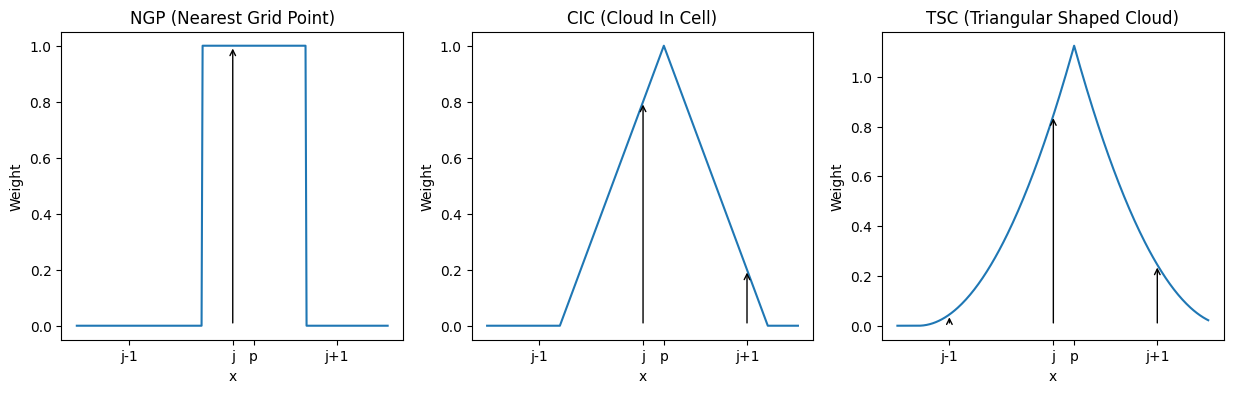
\includegraphics[width=\textwidth]{figures/weight_functions.png}
    \caption{Illustration of three mass assignment schemes—Nearest Grid Point (NGP), Cloud-In-Cell (CIC), and Triangular-Shaped Cloud (TSC)—used to map a particle's mass onto a 1D grid.}
    \label{fig:mass-assignment}
\end{figure}
\begin{itemize}
    \item \textbf{Nearest Grid Point (NGP):} Each particle is assigned entirely to the nearest grid point.
    \item \textbf{Cloud-In-Cell (CIC):} Mass is linearly interpolated to the nearest $2^3 = 8$ surrounding grid points.
    \item \textbf{Triangular-Shaped Cloud (TSC):} Mass is distributed to the nearest $3^3 = 27$ grid points using a quadratic interpolation function.
\end{itemize}

In Fourier space, these mass assignment window functions are represented as:
\begin{equation}
    W(\mathbf{k}) = \prod_{i=1}^{3} W(k_i),
\end{equation}
where
\begin{equation}
    W(k_i) = \left[\frac{\sin\left(\pi k_i / (2 k_N)\right)}{\pi k_i / (2 k_N)}\right]^p,
\end{equation}
with $k_N$ being the Nyquist wavenumber, $k_i$ the $i$-th component of the wavevector $\mathbf{k}$, and $p = 1$ for NGP, $p = 2$ for CIC, and $p = 3$ for TSC \citep{1981csup.book.....H, 2008ApJ...687..738C}.

\subsection{Parallelization Techniques}

Parallelization techniques are pivotal for accelerating computations in large-scale simulations by leveraging multiple processors or computing nodes. The primary strategies include:

\begin{itemize}
    \item \textbf{Domain Decomposition:} The computational domain is partitioned into smaller subdomains, each assigned to a separate processor \citep{1986Natur.324..446B}.
    \item \textbf{Task Parallelism:} Independent tasks are distributed across multiple processors.
    \item \textbf{Data Parallelism:} Identical operations are performed concurrently on different data elements, enabling SIMD (Single Instruction, Multiple Data) execution.
\end{itemize}

These parallelization strategies can be combined to maximize computational efficiency.

\subsection{Adaptive Mesh Refinement}

Adaptive Mesh Refinement (AMR) dynamically adjusts the resolution of the computational grid in regions requiring higher accuracy. The primary goal of AMR is to allocate computational resources efficiently by refining the mesh where necessary and coarsening it elsewhere. AMR generates a hierarchy of refined grids, where each level has finer resolution \citep{1989JCoPh..82...64B}.

Refinement is typically based on physical quantities such as density gradients. For a scalar field $\phi(\mathbf{x})$, refinement is triggered where:
\begin{equation}
    \left| \nabla \phi(\mathbf{x}) \right| > \theta,
\end{equation}
with $\theta$ being a predefined threshold.
\begin{figure}
    \centering
    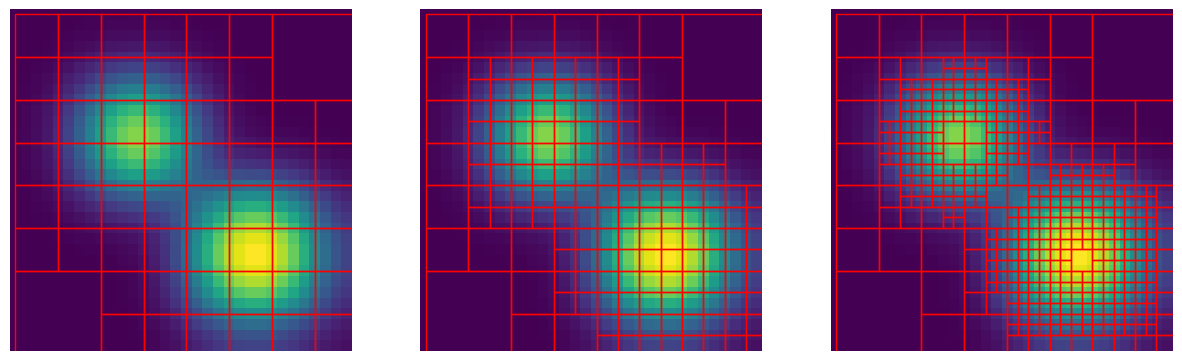
\includegraphics[width=\textwidth]{figures/adaptive_mesh_refinement.png}
    \caption{Illustration of adaptive mesh refinement (AMR) applied to a 2D image with two Gaussian kernels. The left panel shows the initial coarse grid structure over the image. The middle and right panels demonstrate progressively finer levels of mesh refinement in regions of higher intensity, where the Gaussian kernels are located. The red grid outlines indicate the adaptively refined mesh hierarchy, ensuring higher resolution where needed while maintaining computational efficiency in lower-intensity regions.}
    \label{fig:amr}
\end{figure}
Figure~\ref{fig:amr} demonstrates the application of Adaptive Mesh Refinement (AMR) to a two-dimensional image containing two Gaussian kernels. Initially, a uniformly coarse grid overlays the entire image (left panel). As the refinement process progresses, the mesh becomes increasingly finer in regions with higher intensity, specifically around the Gaussian kernels (middle and right panels). The red grid lines represent the hierarchy of the refined meshes, enabling higher resolution where it is most needed and optimizing computational resources by keeping a coarser grid in less significant areas.

\subsection{Tree Construction}

Tree-based data structures are fundamental for efficiently organizing and querying hierarchical spatial data. In computational simulations, the Barnes-Hut Octree is commonly used for tasks like force calculations in $N$-body simulations \citep{1986Natur.324..446B}.

\subsubsection{Barnes-Hut Octree}

The Barnes-Hut algorithm employs an Octree to hierarchically partition the simulation space. Each node represents a cubic region, recursively subdivided into eight octants if it contains more than one particle.

The force on a particle is computed by approximating distant clusters of particles as single mass points. This approximation is controlled by the opening angle $\theta$:
\begin{equation}
    \frac{s}{d} < \theta,
\end{equation}
where $s$ is the size of the node, and $d$ is the distance from the particle to the node's center of mass. This method reduces the computational complexity from $\mathcal{O}(N^2)$ to $\mathcal{O}(N \log N)$.
Figure~\ref{fig:barnes-hut} illustrates the application of the Barnes-Hut Octree algorithm to partition a three-dimensional simulation space containing four particles. 
\begin{figure}[ht]
    \centering
    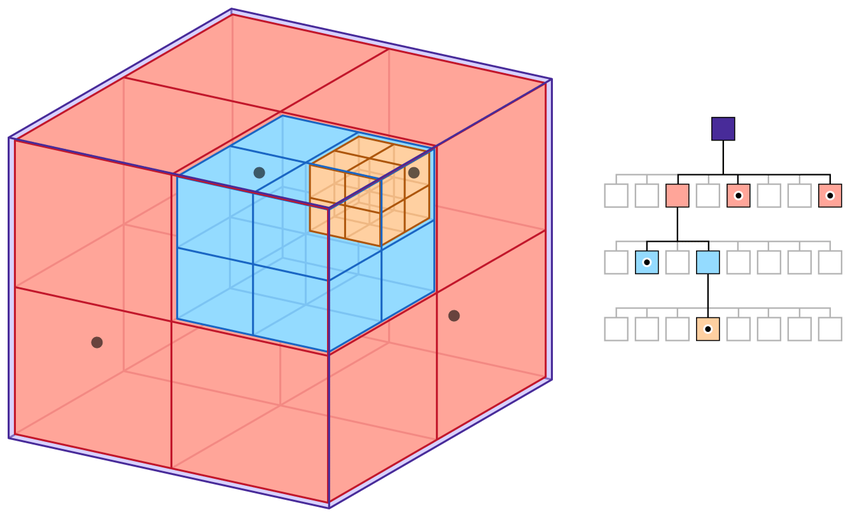
\includegraphics[width=0.6\textwidth]{figures/Octree.png}
    \caption{Illustration of an Octree decomposition for a 3D volume containing four particles. The left panel showcases the spatial subdivision of the volume into hierarchical grid cells, with color-coding indicating different levels of refinement—red for coarse, blue for intermediate, and orange for fine cells where particles reside. The right panel presents the corresponding Octree data structure, highlighting the hierarchical relationships between nodes. The root node (purple) represents the entire simulation volume, while the second layer comprises various node types: empty nodes are depicted in white, single-particle nodes in orange-pink with a black dot, and multi-particle nodes in orange-pink without a dot, which require further subdivision. This hierarchical decomposition enables efficient computation by concentrating resolution in regions with higher particle density while conserving computational resources in less populated areas. Credit by \citet{Powell2023}}
    \label{fig:barnes-hut}
\end{figure}

\subsubsection{Parallel Implementation}

Parallel tree construction involves building local trees within each subdomain and integrating them for global computations \citep{DUBINSKI1996133}. Efficient parallelization enhances scalability and performance in large-scale simulations.

\section{\texttt{FASTPM}}
\texttt{FASTPM} (Fast Particle Mesh; \citealt{10.1093/mnras/stw2123}) is an advanced N-body simulation code tailored for efficiently modeling the evolution of dark matter and halo structures on cosmological scales. Building upon the foundational Particle-Mesh (PM) approach, \texttt{FASTPM} integrates modified kick and drift factors derived from the Zel'dovich Approximation (ZA). This enhancement allows \texttt{FASTPM} to achieve high accuracy in large-scale structure formation while significantly reducing computational overhead. This subsection delineates the core methodology of FASTPM, incorporating the mathematical formalism of its modified kick and drift factors.

\subsection{Modified Kick and Drift Factors}
The cornerstone of \texttt{FASTPM}'s enhanced performance lies in its \textbf{modified kick ($K_{\text{FASTPM}}$)} and \textbf{drift ($D_{\text{FASTPM}}$)} factors. These factors are meticulously derived from the Zel'dovich Approximation (ZA), a first-order Lagrangian perturbation theory (1LPT), to rectify inaccuracies in large-scale growth inherent in standard PM solvers, especially when operating with a limited number of time steps.

First, the Zel'dovich equation of motion to the first order is defined as:
\begin{eqnarray}
    \mathbf{x}_{\text{ZA}}(a) &=& \mathbf{q} + D(a)\mathbf{s}_1,  \nonumber \\
    \mathbf{p}_{\text{ZA}}(a) &=& a^3 E(a) g_p(a) \mathbf{s}_1,  \nonumber \\
    \mathbf{f}_{\text{ZA}}(a) &=& a^2 E(a) g_f(a) \mathbf{s}_1, 
\end{eqnarray}
where $E(a) = \frac{H(a)}{H(a=1)}$ is the dimensionless Hubble parameter, and $g_p(a)$ and $g_f(a)$ are auxiliary factors defined as:
\begin{eqnarray}
    g_p(a)  &=& \frac{dD}{da},  G_p(a) = D(a) \\[0.5em]
    g_f(a)  &=& \frac{d(a^3 E g_p)}{da}, G_f(a) = a^3 E g_p(a)
\end{eqnarray}
The ZA equations of motion are reformulated in terms of drift and kick operators by integrating over a time step from $a_0$ to $a_1$ and eliminating the ZA displacement $\mathbf{s}_1$:
\begin{eqnarray}
    \Delta \mathbf{x}_{\text{ZA}} &=& \mathbf{x}_{\text{ZA}}(a_1) - \mathbf{x}_{\text{ZA}}(a_0) \nonumber \\
    &=& \left[ D(a) \right]_{a_0}^{a_1} \mathbf{s}_1 \nonumber \\
    &=& \frac{\mathbf{p}_{\text{ZA}}(a_r)}{a_r^3 E(a_r)} \left( \frac{\Delta G_p}{g_p(a_r)} \right),
\end{eqnarray}
\begin{eqnarray}
    \Delta \mathbf{p}_{\text{ZA}} &=& \mathbf{p}_{\text{ZA}}(a_1) - \mathbf{p}_{\text{ZA}}(a_0) \nonumber \\
    &=& \frac{\mathbf{f}_{\text{ZA}}(a_r)}{a_r^2 E(a_r)} \left( \frac{\Delta G_f}{g_f(a_r)} \right),
\end{eqnarray}
where $\Delta \mathbf{x}_{\text{ZA}}$ is the change in displacement over the time step, $\Delta \mathbf{p}_{\text{ZA}}$ is the change in momentum over the time step, $a_r$ is a reference scale factor within the time step, $\Delta G_p = G_p(a_1) - G_p(a_0)$, and $\Delta G_f = G_f(a_1) - G_f(a_0)$.
Therefore, the modified kick and drift factors in FASTPM are defined as:
\begin{eqnarray}
    \mathcal{D}_{\text{FASTPM}} &=& \frac{\Delta \mathbf{x}_{\text{ZA}}}{\mathbf{p}_{\text{ZA}}} 
        = \frac{1}{a_r^3 E(a_r)} \left( \frac{\Delta G_p}{g_p(a_r)} \right) \\[1em]
    \mathcal{K}_{\text{FASTPM}} &=& \frac{\Delta \mathbf{p}_{\text{ZA}}}{\mathbf{f}_{\text{ZA}}} 
        = \frac{1}{a_r^2 E(a_r)} \left( \frac{\Delta G_f}{g_f(a_r)} \right) 
\end{eqnarray}
These operators ensure the exact integration of the ZA equations of motion, thereby accurately capturing the linear growth of structures within each time step.

\subsection{Algorithm Steps}
For each simulation time step $t$, \texttt{FASTPM} executes the following sequence of computational procedures to update particle positions and velocities accurately:

\begin{enumerate}
    \item \textbf{Assign Particles to Grid:} 
    \label{fastpm:assign-grid}
    Particles are assigned to a computational grid using an interpolation kernel $W(\mathbf{x} - \mathbf{r}_i)$. This step transforms the discrete particle distribution into a continuous density field suitable for solving Poisson's equation.
    \[
    \rho(\mathbf{x}) = \sum_i m_i W(\mathbf{x} - \mathbf{r}_i)
    \]
    
    \item \textbf{Compute Density Field:}
    Utilizing the assigned grid, compute the density field $\rho(\mathbf{x})$ by summing the contributions of all particles through the interpolation kernel.
    
    \item \textbf{Solve Poisson's Equation:}
    \label{fastpm:poisson}
    Solve Poisson's equation on the grid to obtain the gravitational potential $\Phi(\mathbf{x})$:
    \[
    \nabla^2 \Phi = 4\pi G \rho
    \]
    
    \item \textbf{Compute Gravitational Forces:}
    Calculate the gravitational acceleration $\mathbf{g}(\mathbf{x})$ by taking the gradient of the potential:
    \[
    \mathbf{g}(\mathbf{x}) = -\nabla \Phi
    \]
    
    \item \textbf{Apply Modified Operators:}
    \label{fastpm:modified-kick-drift}
    Utilize the modified kick ($K_{\text{FASTPM}}$) and drift ($D_{\text{FASTPM}}$) factors to update particle velocities and positions. These factors, derived from the ZA, ensure accurate linear growth:
    
    \begin{enumerate}
        \item \textbf{Kick Step:}
        Update particle velocities by applying the gravitational acceleration scaled by the modified kick factor:
        \[
        \mathbf{v}_i\left(t + \frac{\Delta t}{2}\right) = \mathbf{v}_i(t) + \mathbf{g}_i(t) \cdot K_{\text{FASTPM}} \cdot \Delta t
        \]
        
        \item \textbf{Drift Step:}
        Update particle positions using the updated velocities and the modified drift factor:
        \[
        \mathbf{r}_i(t + \Delta t) = \mathbf{r}_i(t) + \mathbf{v}_i\left(t + \frac{\Delta t}{2}\right) \cdot D_{\text{FASTPM}} \cdot \Delta t
        \]
        
        \item \textbf{Second Kick Step:}
        Apply another kick to update velocities to the full time step:
        \[
        \mathbf{v}_i(t + \Delta t) = \mathbf{v}_i\left(t + \frac{\Delta t}{2}\right) + \mathbf{g}_i(t + \Delta t) \cdot K_{\text{FASTPM}} \cdot \Delta t
        \]
    \end{enumerate}
    
    \item \textbf{Update Particle States:}
    Finalize the update of particle velocities and positions after applying the modified kick and drift operators:
    \[
    \mathbf{v}_i(t + \Delta t) = \mathbf{v}_i\left(t + \frac{\Delta t}{2}\right) + \mathbf{g}_i(t + \Delta t) \cdot K_{\text{FASTPM}} \cdot \Delta t
    \]
    \[
    \mathbf{r}_i(t + \Delta t) = \mathbf{r}_i(t) + \mathbf{v}_i\left(t + \frac{\Delta t}{2}\right) \cdot D_{\text{FASTPM}} \cdot \Delta t
    \]
    
    \item \textbf{Advance Time:}
    Increment the simulation time by the time step $\Delta t$:
    \[
    t \leftarrow t + \Delta t
    \]
\end{enumerate}